\section{\textbf{WAHRSCHEINLICHKEITSTHEORIE} - Ereignisse und Wahrscheinlichkeiten}
\subsection{Zufallsereignisse}
Der Ausgangspunkt jeder wahrscheinlichkeitstheoretischen Betrachtung ist ein Zufallsvorgang oder Zufallsexperiment (Würfeln, prüfen eines Werkstücks). Einen Zufallsvorgang zeichnet aus, dass es mehrere, \emph{sich gegenseitig ausschließende} Ergebnisse gibt, von dem genau eines Eintreten wird, wobei nicht bekannt ist welches. Die \emph{möglichen} Ergebnisse eines Zufallsvorgang werden mit $\omega$ und die Menge aller Ergebnisse d.h. der \emph{Ergebnisraum} werden als $\Omega$ bezeichnet. Beim Einmaligen Würfeln kann $\omega$  z.B. $\omega = \{2\}$ sein, während $\Omega = \{1, 2, 3, 4, 5, 6\}$ ist. Wenn man beim Würfeln eine 5 oder 6 benötigen um zu gewinnen, ist man daran interessiert, ob das
Ergebnis des Würfelwurfes in einer bestimmten Teilmenge von $\Omega$ liegt, konkret in der Menge $\{5, 6\}$. Diese Teilmengen nennt man \emph{(Zufalls-)Ereignisse} und man sagt, dass ein Ereignis $A \subset \Omega$ eintritt, wenn das Ergebnis $\omega$ des Zufallsvorgang ein Element von A is. Die einelementigen Teilmengen $\{\omega\}$ von $\Omega$ nennt man auch \emph{Elementareereignisse}.\\\\
\textbf{Mengenlehre und wahrscheinlichkeitstheoretische Interpretation}: \emph{Kommutativgesetz}: $A \cap  B = B \cap A$. \emph{Assoziativgesetz}: $(A \cap B ) \cap C = A \cap (B \cap C)$. \emph{Distributivgesetz}: $(A \cup B) \cap C = (A \cap C) \cup (A \cap C)$. \emph{De Morgansche Regel}: $\overline{(A \cap B)} = \bar{A} \cup \bar{B}$ (geht auch, wenn man $\cap$ und $\cup$ vertauscht)\\\\
\textbf{Ereignisfelder}: Die Menge aller Ergebnisse bezeichnet man als \emph{Ereignisfeld} $\mathcal{F}$. Wenn der Ergebnisraum $\Omega$ endlich oder abzählbar unendlich ist, ist die Potenzmenge $\mathcal{P}(\Omega)$ das üblicherweise betrachtete Ereignisfeld. Ist $\Omega$ überabzählbar können als Ereignisfelder nur $\sigma$-Algebren betrachtet werden. Diese sind definiert durch: $\Omega \in \mathcal{F}$,\,\,\,$A \in \mathcal{F} \Rightarrow \bar{A} \in \mathcal{F}$,\,\,\,abzählbar viele Ereignisse $A_1, A_2, ... \in \mathcal{F} \Rightarrow \cup_{i=1}^\infty A_i \in \mathcal{F}$

\subsection{Laplace-Wahrscheinlichkeiten und Kombinatorik}
\begin{wrapfigure}{r}{0.4\textwidth}
    \vspace{-6mm}
    \centering
    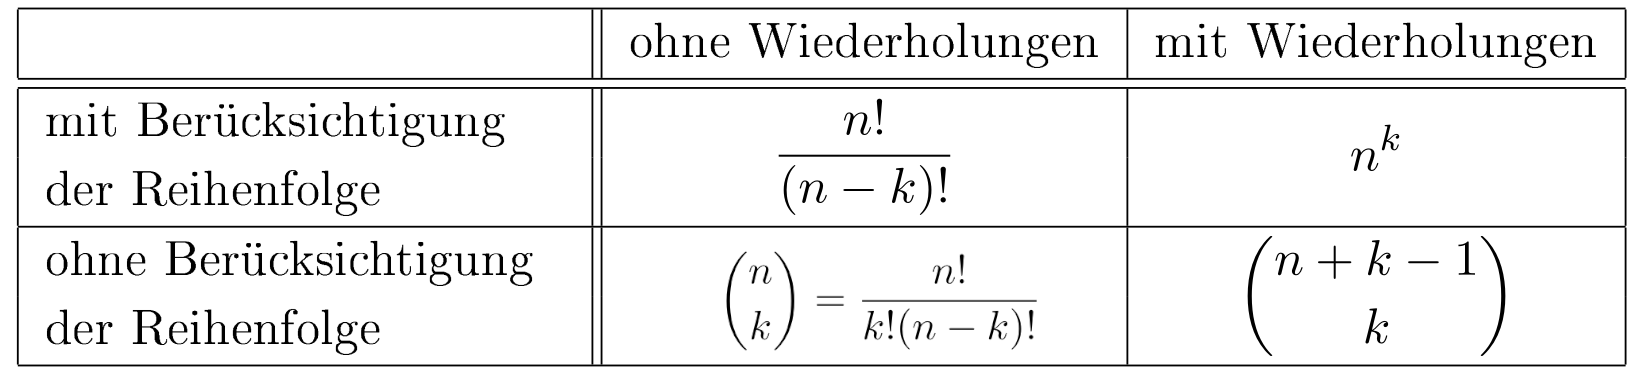
\includegraphics[width=0.4\textwidth]{images/wiederholung_kombinatorik.png}
    \caption{Kombinatorik Wiederholung}
    \vspace{-6mm}
    \label{fig:}
\end{wrapfigure}
\textbf{Laplace-Wahrscheinlichkeit}: $P(A) = \frac{\text{Anzahl der für $A$ günstigen Ergebnisse}}{\text{Anzahl aller möglichen Ergebnisse}} = \frac{|A|}{|\Omega|}$. Bsp. die Wahrscheinlichkeit eine ungerade Zahl zu würfeln: $P(A) = \frac{|\{1,3,5\}|}{|\{1,2,3,4,5,6\}|} = \frac{3}{6} = \frac{1}{2}$

\textbf{Permutation}: Anordnen von n unterscheidbaren Objekten: $n \cdot (n-1) \cdot (n-2) ... = \Pi_{i=1}^n i = n!$. Bsp: Sitzordnung an einem Tisch.\,\,\,\,\textbf{Variation ohne Wiederholungen}: Möglichkeiten k aus n unterscheidbaren Objekten \emph{mit} Berücksichtigung der Reihenfolge auszuwählen. Formel 1 Siegertreppchen Anordnungen bei 20 Teilnehmern.\,\,\,\,\textbf{Variation mit Wiederholungen}: Bsp. k mal ziehen aus n Möglichkeiten. Bsp: Kombinationen bei Passwörtern.\,\,\,\,\textbf{Kombination ohne Wiederholungen} Ziehen von k aus n Objekten. Die Reihenfolge spielt keine Rolle. Bsp: \hlc{Lotto} 6 aus 49.\,\,\,\,\textbf{Kombination mit Wiederholungen}: Die Anzahl Kombinationen beim Auswählen von k Objekten aus n unterscheidbaren Objekten.
\subsection{Wahrscheinlichkeitsmaße}
\textbf{Definition Wahrscheinlichkeitsmaß}: Es sei $\Omega$ der Ergebnisraum eines Zufallsvorgangs und $\mathcal{F}$ ein Ereignisfeld über $\Omega$. Eine Abbildung $P$ die jedem Ereignis $A \in \mathcal{F}$ eine reelle Zahl zuordnet: $P: \mathcal{F} \rightarrow \mathds{R}$ mit $A \mapsto P(A)$ nennt man \emph{Wahrscheinlichkeitsmaß} auf $\mathcal{F}$ wenn sie die Axiome von Kolmogoroff erfüllt: \textbf{K1} $P(A) \ge 0$ (Nichtnegativität).\,\,\,\,\textbf{K2} $P(\Omega) = 1$ (Normierung).\,\,\,\,\textbf{K3} Falls $A \cap B = \emptyset$, so ist $ (A \cup B) = P(A) + P(B)$ (Additivität).\\
Daraus folgen folgende Rechenregel:\,\,\,\,(\textbf{i}) $0 \le P(A) \le 1$.\,\,\,\,(\textbf{ii}) $P(\emptyset) = 0$.\,\,\,\,(\textbf{iii}) $P(A) \le P(B)$, falls $A \subset B$.\,\,\,\,(\textbf{iv}) $P(\bar{A}) = 1 - P(A)$.\,\,\,\,(\textbf{v}) $P(A_1\cup ... \cup A_k) = P(A_1) + ... + P(A_k)$ falls $A_1, ..., A_k$ paarweise disjunkt. $\Rightarrow$ $P(A) = \sum_{w \in A}P(\{\omega\}.$\,\,\,\,(\textbf{vi}) $P(B \backslash A) = P(B) - P(A \cap B)$.\,\,\,\,(\textbf{vii}) $P(A\cup B) = P(A) + P(B) - P(A \cap B)$ (Additionssatz)
\subsection{Bedingte Wahrscheinlichkeiten und unabhängige Ereignisse}
\section{Diskrete Zufallsvariablen}
\section{Stetige Zufallsvariablen}
\section{Gesetz der großen Zahlen und zentraler Grenzwertsatz}
\section{Zufallsvektoren}
